\chapter{Spatial Decomposition}{\label{ch:Spatial Decomposition}
  \def\figpath{chapters/05/figures/}
  \graphicspath{ {\figpath} }
  %%%%%%%%%%%%%%%%%%%%%%%%%%%%%%%%%%%%%%%%%%%%%%%%%%%%%%%%%%%%%%%%%%%%%%%%%%%%%%
  % Introduction
  %%%%%%%%%%%%%%%%%%%%%%%%%%%%%%%%%%%%%%%%%%%%%%%%%%%%%%%%%%%%%%%%%%%%%%%%%%%%%%
  \section{Introduction}{\label{sec:Spatial Decomposition:Introduction}
    Until relatively recently, the method of choice for neutronics calculations has been neutron diffusion.
    Neutron diffusion codes can perform whole-core calculations, on a typical workstation, in relatively short run-times.
    However, with the recent shift towards higher fidelity methods such as \ac{SN}, and \ac{MOC} \cite{Askew1972}, more significant computational resources are necessary.
    These high fidelity methods allow for more detailed analysis, through finer resolution and use of fewer approximations, but typically take far more time to perform calculations; particularly for large calculations.
    Although processor clock-speeds have significantly improved, in the past several years processors have, for the most part, not gotten faster.
    To reduce the run-times (real-time) of high fidelity simulations, it is thus necessary to rely on parallelism.

    There are many different aspects of parallelism, and thread-based parallelism has been discussed previously \cref{sec:MOC:Parallelism}.
    This type of parallelism (thread), is limited to the resources of a single computational node.
    In order to utilize more resources, it is necessary to use a technique called \emph{domain decomposition}.
    Even without considerations for run-times, these high-fidelity simulations typically use more memory than is available on a single node, and domain decomposition becomes a necessity.
    In general, domain decomposition involves splitting up one domain of the problem into smaller subdomains; some typical domains to decompose are space, direction, and energy.
    Each smaller subdomain is assigned to a separate processor, and these can be run in parallel; although, there is generally some communication between the processors.

    In Monte-Carlo simulations, it is common that spatial decomposition involves duplication of some spatial locations [CITATION].
    However, in deterministic transport methods, each domain is typically \emph{partitioned}, that is the domain is split without any overlap between subdomains.
    The MPACT \cite{MPACT2016} code has the ability to decompose two domains: space and direction.
    In MPACT, each discrete direction has a calculable amount of work, and the decomposition is trivial; in general, the same cannot be said of the spatial domain.
    This chapter focuses on improvements to the spatial decomposition techniques used in MPACT; these techniques, however, can be applied to other transport codes and similar results would be expected.
    The contents of this chapter are, in large part, adapted from an article published on this work \cite{Fitzgerald2019a}.

    As diffusion has been the method of choice for so long in the reactor physics field, spatial partitioning techniques common in other fields have, largely, not been applied.
    Transport codes such as MPACT \cite{MPACT2016}, or OpenMOC \cite{Gunow2018} used simple spatial partitioning methods that divided the core into uniformly sized blocks.
    However, the spatial partitioning of a reactor can be abstracted to a graph partitioning problem \cite{Fitzgerald2017}, which has been well studied in computer science \cite{Elsner1997} and applied to other simulation fields such as computational fluid dynamics \cite{Yao1998}.
    In general, the graph partitioning problem is NP-complete, meaning that a partitioning cannot be easily verified as optimal; therefore, graph partitioning relies on approximate heuristic methods.
    Many different methods have been developed for graph partitioning, several of which are discussed in \cref{sec:Spatial Decomposition:Applied Graph Theory}.

    The remained of this chapter is structured as follows.
    In \cref{sec:Spatial Decomposition:Spatial Decomposition in MPACT}, a description of spatial decomposition in MPACT is given.
    \Cref{sec:Spatial Decomposition:Applied Graph Theory} introduces relevant graph theory concepts, and the methods used for spatial partitioning in this work.
    \Cref{sec:Spatial Decomposition:Applications for MPACT} describes the applications of these graph theory methods in MPACT.
    \Cref{sec:Spatial Decomposition:Results} compares methods for 2-D and 3-D reactor simulations.
    Finally, \cref{sec:Spatial Decomposition:Conclusions} lists the conclusions that are drawn from this work.
  }
  %%%%%%%%%%%%%%%%%%%%%%%%%%%%%%%%%%%%%%%%%%%%%%%%%%%%%%%%%%%%%%%%%%%%%%%%%%%%%%
  % Spatial Decomposition in MPACT
  %%%%%%%%%%%%%%%%%%%%%%%%%%%%%%%%%%%%%%%%%%%%%%%%%%%%%%%%%%%%%%%%%%%%%%%%%%%%%%
  \section{Spatial Decomposition in MPACT}{\label{sec:Spatial Decomposition:Spatial Decomposition in MPACT}
    MPACT is a neutron transport code, based on the \ac{MOC}.
    It was originally developed for direct whole-core simulation of \acp{LWR}.
    In the \ac{MOC}, an approximate transport equation is solved analytically along characteristic rays that traverse the problem.
    By using many of these characteristic rays, an accurate solution is obtained; however, storing the data of these characteristic rays can use a considerable amount of memory.

    In MPACT, the modular ray-tracing technique \cite{Saji2000} is used to reduce the memory used for storing characteristic ray information.
    Modular ray-tracing involves dividing the reactor system into \emph{ray-tracing modules}, which are small geometries that are often repeated in the reactor.
    Characteristic rays are constructed in each ray-tracing module such that each ray directly links to a ray in an adjacent module.
    In this method, characteristic ray information is only stored for each \emph{unique} ray-tracing module.

    Ray-tracing modules are the smallest unit for spatial decomposition in MPACT \cite{StimpsonPartitioning2017}.
    These ray-tracing modules are typically an axial slice of a quarter of a full fuel assembly, as shown in \cref{fig:Spatial Decomposition:5a-2d abstraction}
    The core consists of a structured grid of these modules in which each module has the same dimensions but may have different numbers of computational cells.
    Therefore, in MPACT, the spatial decomposition is a structured grid partitioning problem.

    In general, it is possible to use the computational cells as the smallest unit in the decomposition.
    However, this causes the decomposition problem to become an unstructured mesh partitioning problem.
    This is not done in MPACT because communication would become significantly more complicated.
    Additionally, there would be more re-entrant rays which would have negative impacts on the rate of convergence.

    \begin{figure}
      \centering
      \begin{subfigure}[t]{0.45\textwidth}
        \centering
        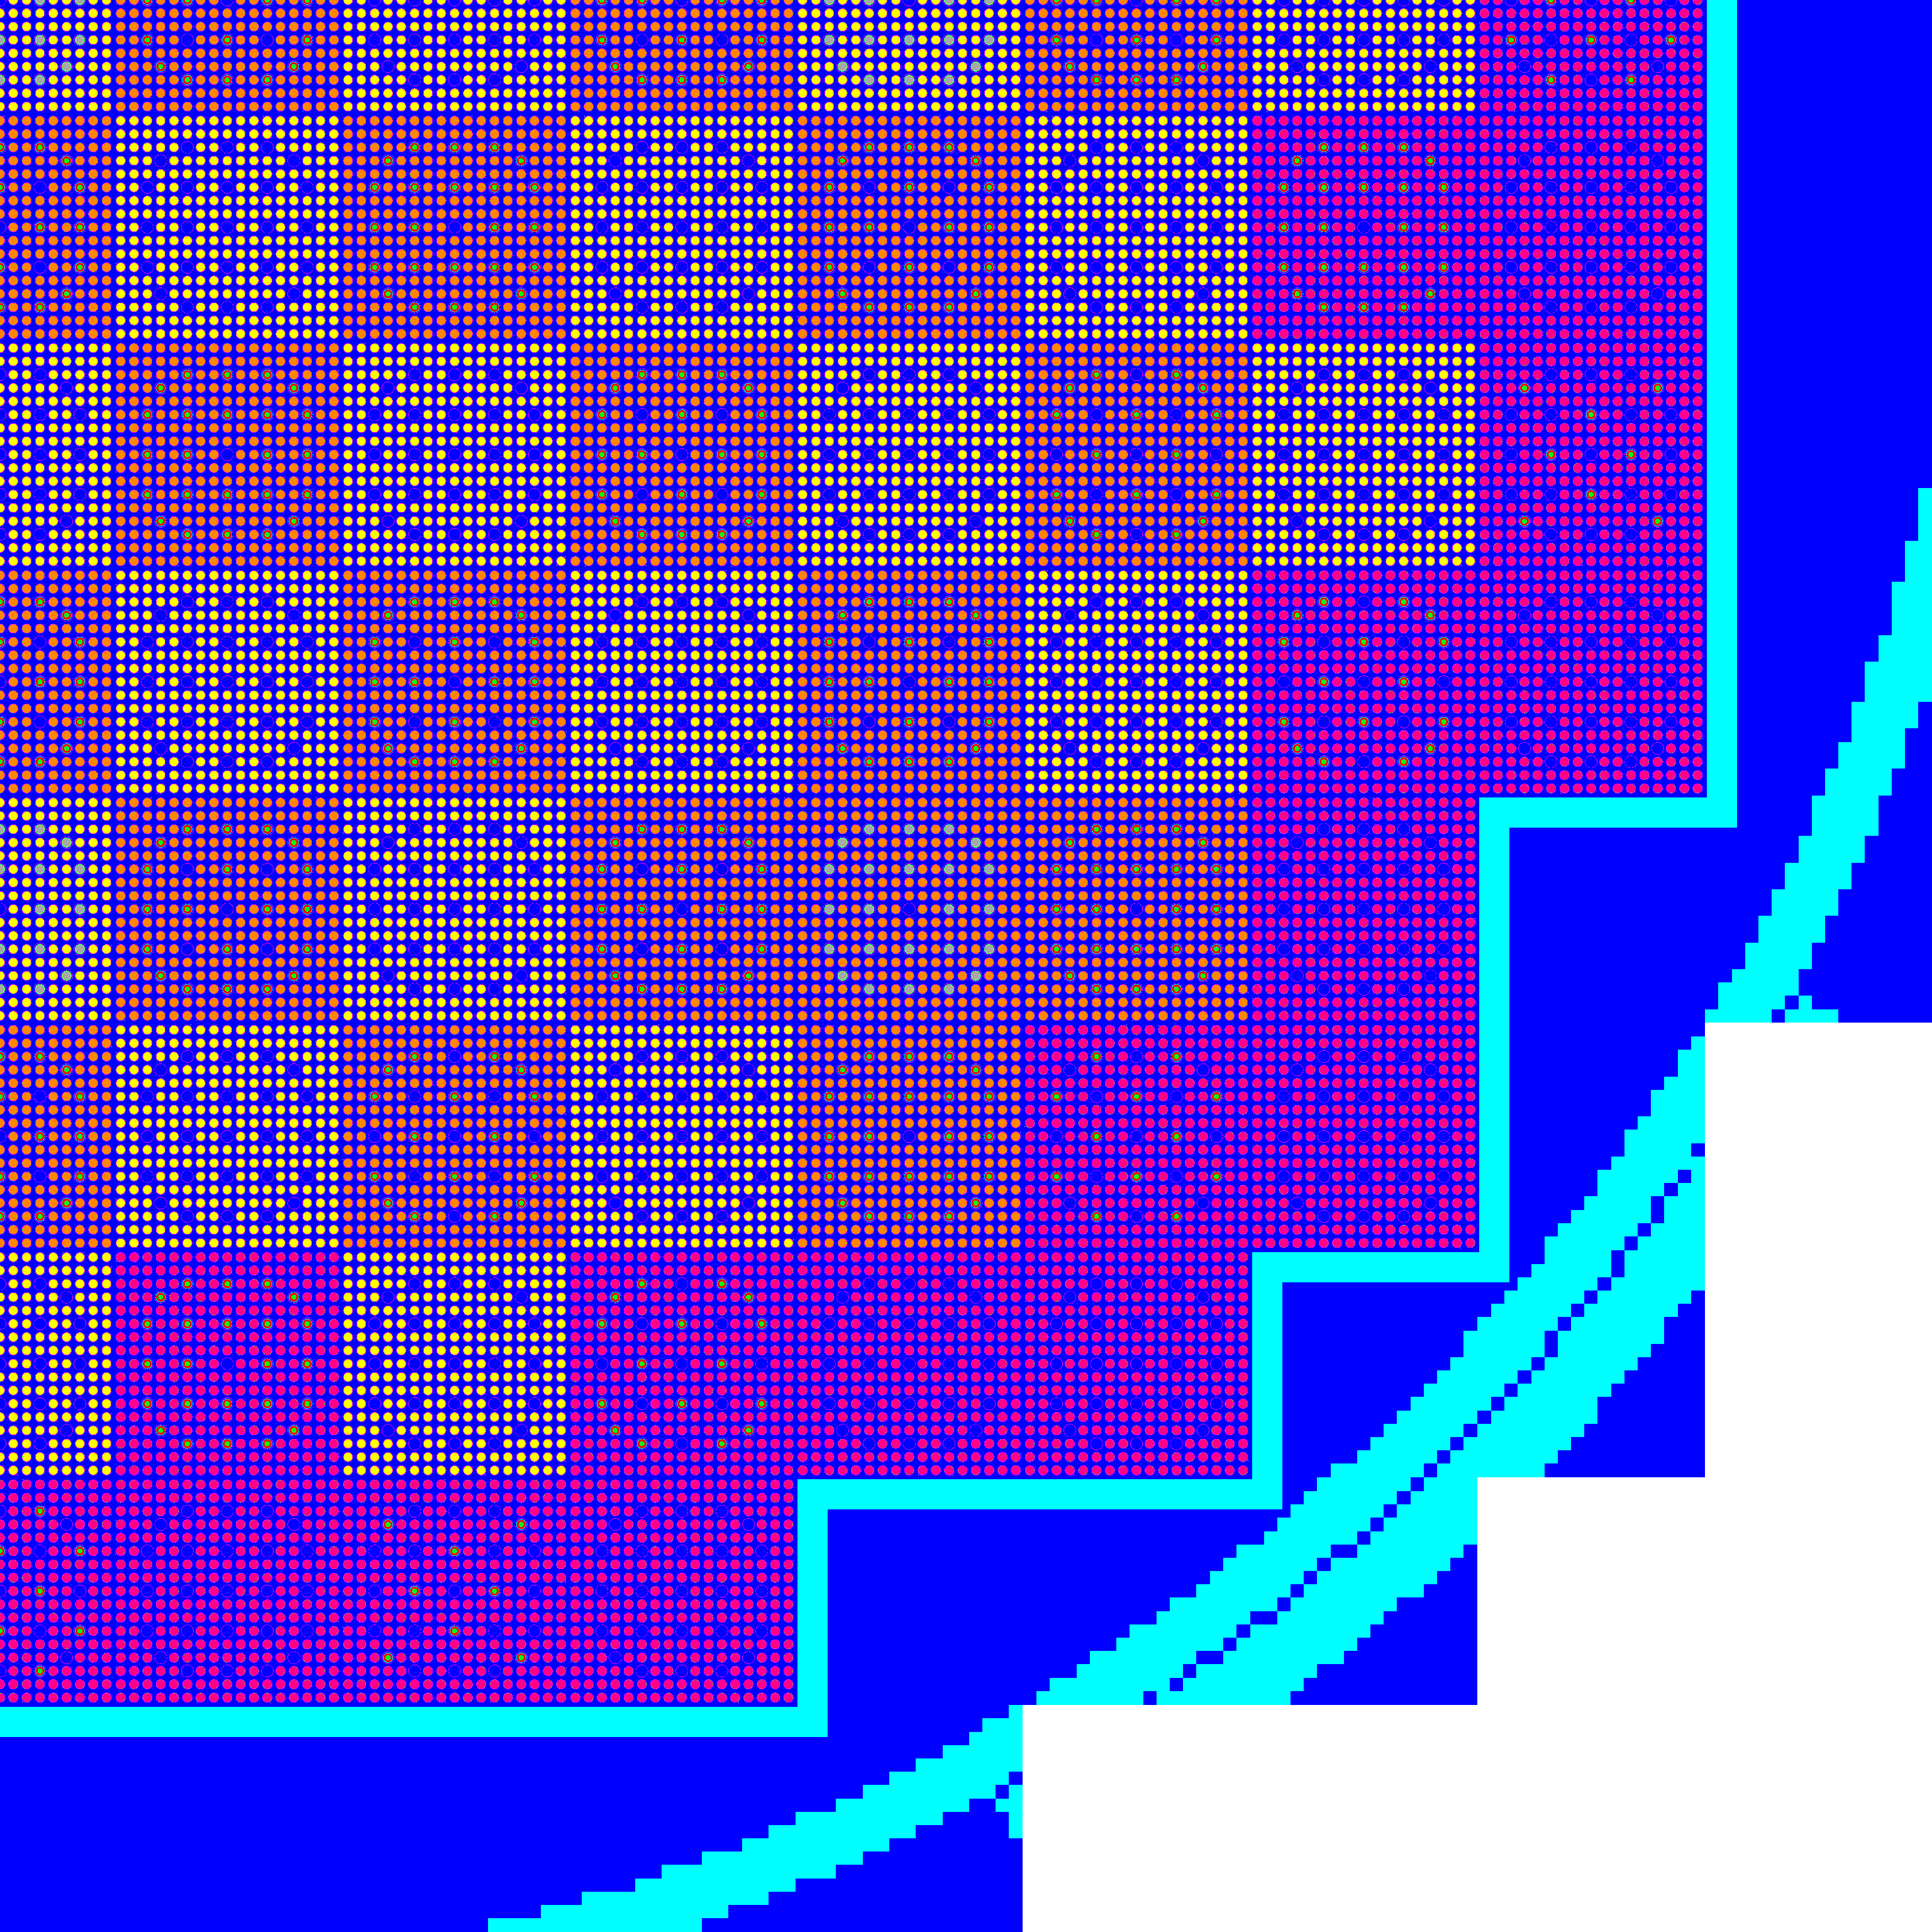
\includegraphics[width=0.9\textwidth]{5a-2d_core}
        \caption{fine mesh\label{fig:Spatial Decomposition:5a-2d configuration}}
      \end{subfigure}%
      ~
      \begin{subfigure}[t]{0.45\textwidth}
        \centering
        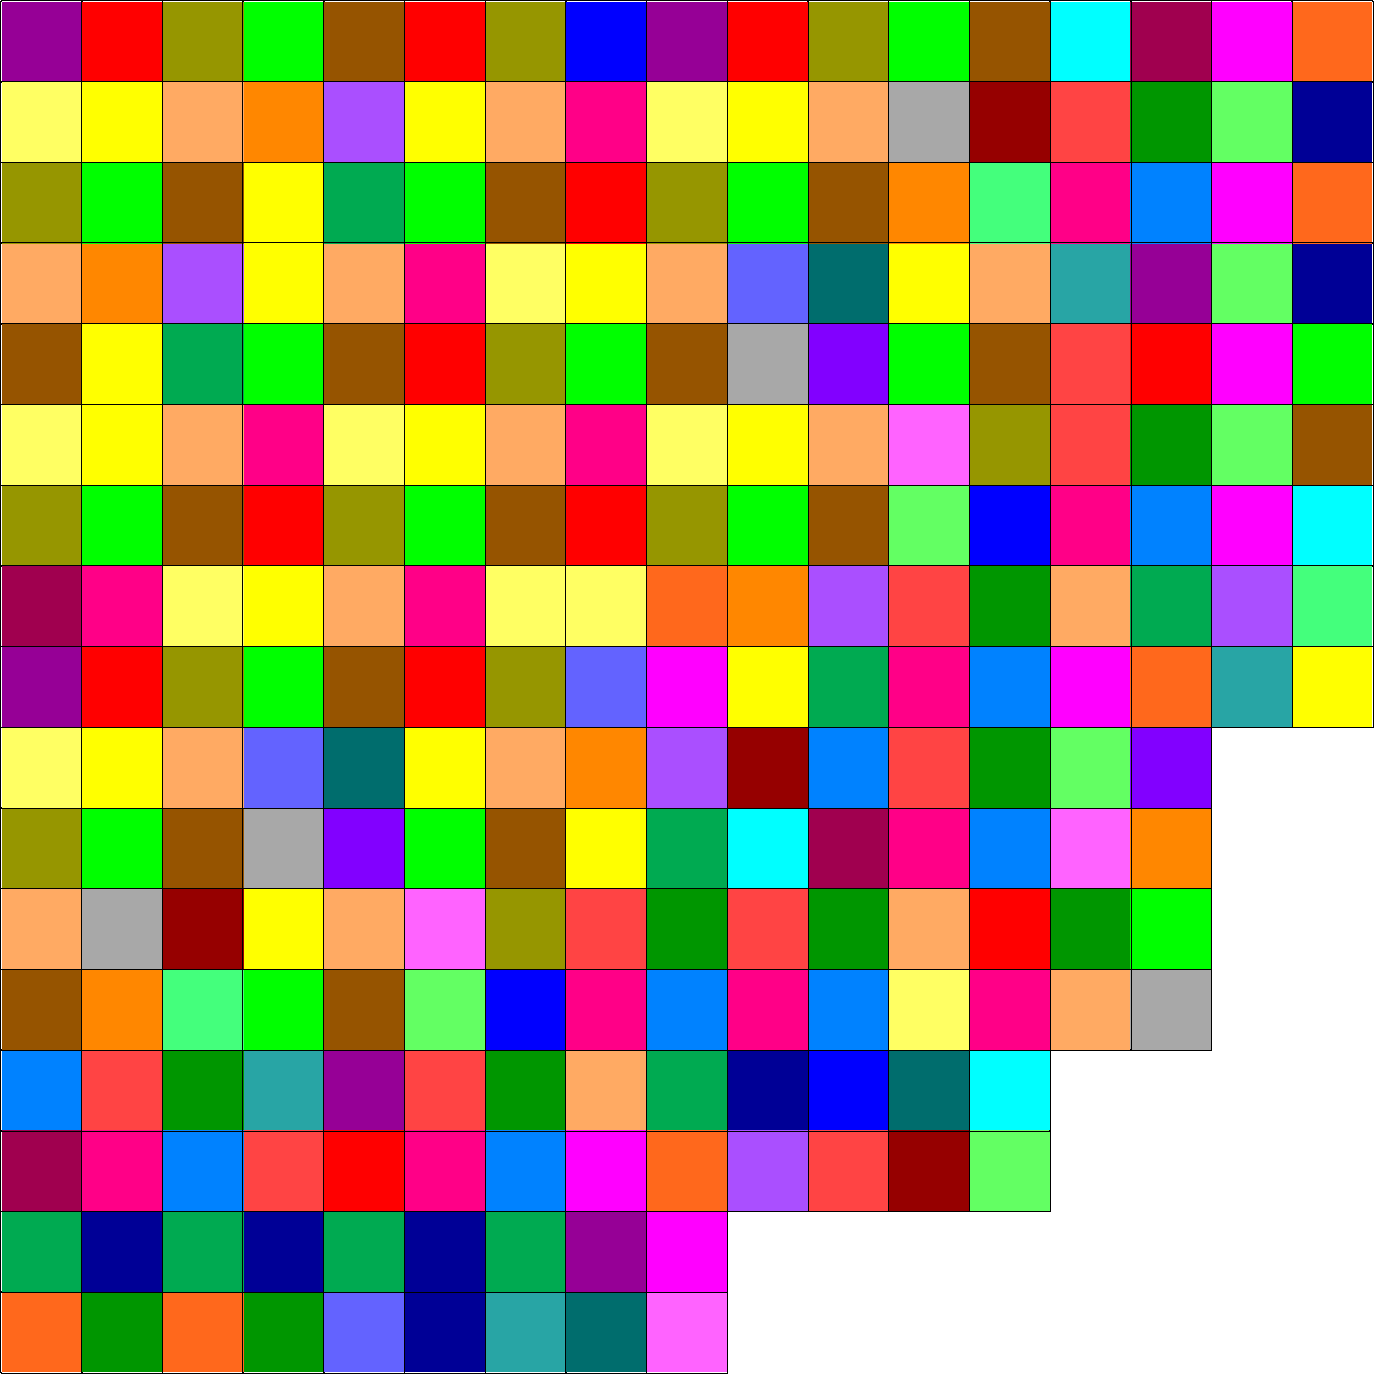
\includegraphics[width=0.9\textwidth]{modmesh_5a-2d}
        \caption{ray-tracing module mesh\label{fig:Spatial Decomposition:5a-2d modular mesh}}
      \end{subfigure}
      \caption{Example quarter core configuration and corresponding ray-tracing modular mesh in MPACT. \label{fig:Spatial Decomposition:5a-2d abstraction}}
    \end{figure}

    MPACT has had two spatial decomposition methods in the past: manual decomposition, and assembly-based decomposition.
    A user may manually enter a decomposition \cite{StimpsonPartitioning2017}, but it is time consuming to construct a balanced decomposition and will likely still be suboptimal to some degree.
    An automated method exists that recursively bisects the core using Morton-ordering \cite{Morton1966} applied to the reactor assembly geometries.
    While this method is automated, it often yields very imbalanced domains, and also restricts the number of subdomains that can be used.

    Previous work has shown that spatial decomposition of reactors can be abstracted to a graph partitioning problem \cite{Fitzgerald2017}.
    The use of graph partitioning methods in MPACT is expected to solve the issues encountered in each of the two approaches described above.
    These methods can be used to decompose into an arbitrary number of domains with high quality results, without user input.

    Existing graph partitioning libraries such as METIS \cite{METIS} partition graphs very efficiently and have very high quality results.
    To use all given processors, MPACT requires that each spatial subdomain contains at least one module, i.e. no partition can be empty.
    However, in some cases, particularly when the number of partitions is high, METIS may generate empty partitions.
    This means METIS cannot be used to decompose the core into an arbitrary number of subdomains without modifying the resulting partitions.
    For this reason, MPACT does not rely on third-party libraries for graph partitioning in the spatial decomposition process.
  }
  %%%%%%%%%%%%%%%%%%%%%%%%%%%%%%%%%%%%%%%%%%%%%%%%%%%%%%%%%%%%%%%%%%%%%%%%%%%%%%
  % Applied Graph Theory
  %%%%%%%%%%%%%%%%%%%%%%%%%%%%%%%%%%%%%%%%%%%%%%%%%%%%%%%%%%%%%%%%%%%%%%%%%%%%%%
  \section{Applied Graph Theory}{\label{sec:Spatial Decomposition:Applied Graph Theory}
    \blindtext[2]
    %%%%%%%%%%%%%%%%%%%%%%%%%%%%%%%%%%%%%%%%%%%%%%%%%%%%%%%%%%%%%%%%%%%%%%%%%%%%
    % Graph Partitioning Methods
    %%%%%%%%%%%%%%%%%%%%%%%%%%%%%%%%%%%%%%%%%%%%%%%%%%%%%%%%%%%%%%%%%%%%%%%%%%%%
    \subsection{Graph Partitioning Methods}{\label{ssec:Spatial Decomposition:Graph Partitioning Methods}
      \blindtext[2]
      %%%%%%%%%%%%%%%%%%%%%%%%%%%%%%%%%%%%%%%%%%%%%%%%%%%%%%%%%%%%%%%%%%%%%%%%%%
      % Recursive Spectral Bisection
      %%%%%%%%%%%%%%%%%%%%%%%%%%%%%%%%%%%%%%%%%%%%%%%%%%%%%%%%%%%%%%%%%%%%%%%%%%
      \subsubsection{Recursive Spectral Bisection}{\label{sssec:Spatial Decomposition:Recursive Spectral Bisection}
        \blindtext[4]
      }
      %%%%%%%%%%%%%%%%%%%%%%%%%%%%%%%%%%%%%%%%%%%%%%%%%%%%%%%%%%%%%%%%%%%%%%%%%%
      % Recursive Inertial Bisection
      %%%%%%%%%%%%%%%%%%%%%%%%%%%%%%%%%%%%%%%%%%%%%%%%%%%%%%%%%%%%%%%%%%%%%%%%%%
      \subsubsection{Recursive Inertial Bisection}{\label{sssec:Spatial Decomposition:Recursive Inertial Bisection}
        \blindtext[4]
      }
      %%%%%%%%%%%%%%%%%%%%%%%%%%%%%%%%%%%%%%%%%%%%%%%%%%%%%%%%%%%%%%%%%%%%%%%%%%
      % Recursive Expansion-Based Methods
      %%%%%%%%%%%%%%%%%%%%%%%%%%%%%%%%%%%%%%%%%%%%%%%%%%%%%%%%%%%%%%%%%%%%%%%%%%
      \subsubsection{Recursive Expansion-Based Methods}{\label{sssec:Spatial Decomposition:Recursive Expansion-Based Methods}
        \blindtext[8]
      }
    }
  }
  %%%%%%%%%%%%%%%%%%%%%%%%%%%%%%%%%%%%%%%%%%%%%%%%%%%%%%%%%%%%%%%%%%%%%%%%%%%%%%
  % Applications for MPACT
  %%%%%%%%%%%%%%%%%%%%%%%%%%%%%%%%%%%%%%%%%%%%%%%%%%%%%%%%%%%%%%%%%%%%%%%%%%%%%%
  \section{Applications for MPACT}{\label{sec:Spatial Decomposition:Applications for MPACT}
    \blindtext[8]
    %%%%%%%%%%%%%%%%%%%%%%%%%%%%%%%%%%%%%%%%%%%%%%%%%%%%%%%%%%%%%%%%%%%%%%%%%%%%
    % CMFD Acceleration
    %%%%%%%%%%%%%%%%%%%%%%%%%%%%%%%%%%%%%%%%%%%%%%%%%%%%%%%%%%%%%%%%%%%%%%%%%%%%
    \subsection{CMFD Acceleration}{\label{ssec:Spatial Decomposition:CMFD Acceleration}
      \blindtext[3]
    }
  }
  %%%%%%%%%%%%%%%%%%%%%%%%%%%%%%%%%%%%%%%%%%%%%%%%%%%%%%%%%%%%%%%%%%%%%%%%%%%%%%
  % Results
  %%%%%%%%%%%%%%%%%%%%%%%%%%%%%%%%%%%%%%%%%%%%%%%%%%%%%%%%%%%%%%%%%%%%%%%%%%%%%%
  \section{Results}{\label{sec:Spatial Decomposition:Results}
    %%%%%%%%%%%%%%%%%%%%%%%%%%%%%%%%%%%%%%%%%%%%%%%%%%%%%%%%%%%%%%%%%%%%%%%%%%%%
    % 2-D Results
    %%%%%%%%%%%%%%%%%%%%%%%%%%%%%%%%%%%%%%%%%%%%%%%%%%%%%%%%%%%%%%%%%%%%%%%%%%%%
    \subsection{2-D Results}{\label{ssec:Spatial Decomposition:2-D Results}
      \blindtext[8]
    }
    %%%%%%%%%%%%%%%%%%%%%%%%%%%%%%%%%%%%%%%%%%%%%%%%%%%%%%%%%%%%%%%%%%%%%%%%%%%%
    % 3-D Results
    %%%%%%%%%%%%%%%%%%%%%%%%%%%%%%%%%%%%%%%%%%%%%%%%%%%%%%%%%%%%%%%%%%%%%%%%%%%%
    \subsection{3-D Results}{\label{ssec:Spatial Decomposition:3-D Results}
      \blindtext[4]
    }
  }
  %%%%%%%%%%%%%%%%%%%%%%%%%%%%%%%%%%%%%%%%%%%%%%%%%%%%%%%%%%%%%%%%%%%%%%%%%%%%%%
  % Conclusions
  %%%%%%%%%%%%%%%%%%%%%%%%%%%%%%%%%%%%%%%%%%%%%%%%%%%%%%%%%%%%%%%%%%%%%%%%%%%%%%
  \section{Conclusions}{\label{sec:Spatial Decomposition:Conclusions}
    \blindtext[4]
  }
}